\documentclass{article}
\usepackage{algorithm}
\usepackage{algorithmicx,algpseudocode}
\usepackage{tikz}
\usepackage{natbib}
\usepackage{graphicx}
\usepackage{amsmath}
\usepackage{authblk}
\newcommand{\be}{\begin{equation}}
\newcommand{\ee}{\end{equation}}
\newcommand{\eps}{\epsilon}

\bibliographystyle{abbrvnat}
\setcitestyle{authoryear,open={(},close={)}}

\begin{document}

%Section 3 in the paper definitely needs one or two paragraphs talking more about the labels. How did we create them, what is the composition of the classes, where do we use prices and where returns. 
%I don't understand figure 3. I don't know what is the x axis. 
%I'm done with the paper version also. The comments for the last part are in the pdf document (in dropbox). 
%There is room for improvement of the paper. As I said we should compare against JIn's results in python. 
%From the finance perspective, I think it would be interesting to see PnL by asset. It would also be good to find patterns for which assets we do well and for each we don't do well. 
%We also only comparing our algorithm vs perfect future information. It would be interesting to compare against other trading strategies (commonly known). 
%Otherwise we can come up with simple strategies: moving averages.




\title{Classification-based Financial Markets Prediction using Deep Neural Networks}

 


%For one neural networks have always under-delivered in the investment manaagement realm because the signal to noise ratio is so bad in this arena and they latch onto noise in any given training set. So, I think many people would be interested. I would think you would want to keep the "this is why it improves forecasting ability" as a front and center point of the paper. The fact you got 61 cores to do anything in unison is very umpressive, but the focus of a finance paper is what problem of interest to researchers and practitioners couldn't be solved well before but can now. In the realm of asset forecasting, distinct factors have always been used to help reduce the signal to noise ratio and make the forecast stable
\author[1]{Matthew Dixon}
\author[2]{Diego Klabjan}
\author[3]{Jin Hoon Bang}
\affil[1]{Stuart School of Business\\
Illinois Institute of Technology\\
10 West 35th Street\\
Chicago, IL 60616\\
matthew.dixon@stuart.iit.edu}
\affil[2]{Department of Financial Engineering\\
Northwestern University\\
Evanston, IL\\
d-klabjan@northwestern.edu}
\affil[3]{Department of Computer Science\\
Northwestern University\\
Evanston, IL\\
jinhoonbang@u.northwestern.edu 
}


%\date{5 May 2013}

\maketitle
\begin{abstract}
Deep neural networks (DNNs) are powerful types of artificial neural networks (ANNs) that use several hidden layers. They have recently gained considerable attention in the speech transcription and image recognition community \citep{krizhevsky2012} for their superior predictive properties including robustness to overfitting. However their application to algorithmic trading has not been previously researched, partly because of their computational complexity. This paper describes the application of DNNs to predicting financial market movement directions. In particular we describe the configuration and training approach and then demonstrate their application to backtesting a simple trading strategy over 45 different Commodity and FX future mid-prices at 5-minute intervals.  All results in this paper are generated using a C++ implementation on the Intel Xeon Phi co-processor which is 11.4x faster than the serial version and a Python strategy backtesting environment both of which are available as open source code written by the authors.

\end{abstract}


%\category{G.4}{MATHEMATICAL SOFTWARE}{Parallel and
%vector implementations}
%\terms{Algorithms, Performance}
%\keywords{Deep Neural Networks, Market Prediction, Intel Xeon Phi}
%motivation
%description of algorithm
%description of parallelization
%performance results
%WFO -> 



\section{Introduction} % literature review
Many of the challenges facing methods of financial econometrics include non-stationarity, non-linearity or noisiness of the time series. While the application of artificial neural networks (ANNs) to time series methods are well documented \citep{Faraway98, Refenes1994,Trippi92,Fkaastra95} their proneness to over-fitting, convergence problems, and difficulty of implementation raised concerns. Moreover, their departure from the foundations of financial econometrics alienated the financial econometrics research community and finance practitioners.

However, algotrading firms employ computer scientists and mathematicians who are able to perceive ANNs as not merely black-boxes, but rather a non-parametric approach to modeling based on minimizing an entropy function. As such, there has been a recent resurgence in the method, in part facilitated by advances in modern computer architecture \citep{Chen2013, Niaki2013, Vanstone2010}.


A deep neural network (DNN) is an artificial neural network with multiple hidden layers of units between the input and output layers. They have been popularized in the artificial intelligence community for their successful use in image classification \citep{krizhevsky2012} and speech recognition. The field is referred to as "Deep Learning".
  
In this paper, we shall use DNNs to partially address some of the historical deficiencies of ANNs. Specifically, we model complex non-linear relationships between the independent variables and dependent variable and reduced tendency to overfit. In order to do this we shall exploit advances in low cost many-core accelerator platform to train and tune the parameters of our model.

For financial forecasting, especially in multivariate forecasting analysis, the feed-forward
topology has gained much more attention and shall be the approach used here. Back-propagation and gradient descent have been the preferred method for training these structures due to the ease of implementation and their tendency to converge to better local optima in comparison with other trained models. However, these methods can be computationally expensive, especially when used to train DNNs. 

There are many training parameters to be considered with a DNN, such as the size (number of layers and number of units per layer), the learning rate and initial weights. Sweeping through the parameter space for optimal parameters is not feasible due to the cost in time and computational resources. We shall use mini-batching (computing the gradient on several training examples at once rather than individual examples) as one common approach to speeding up computation. We go further by expressing the back-propagation algorithm in a form that is amenable to fast performance on an Intel Xeon Phi co-processor \citep{Jeffers2013}. General purpose hardware optimized implementations of the back-propagation algorithm are described in \citep{Shekhar94}, however our approach is tailored for the Intel Xeon Phi co-processor.

The main contribution of this paper is to describe the application of deep neural networks to financial time series data in order to classify financial market movement directions. Traditionally, researchers will iteratively experiment with a handful of signals to train a level based method, such as vector autoregression, for each instrument (see for example \cite{Fkaastra95, Refenes1994, Trippi92}). More recently, however,  \cite{Leung2000} provide evidence that classification based methods outperform level based methods in the prediction of the direction of stock movement and trading returns maximization. 

Using 5 minute interval prices from June 1989 to March 2013,  our approach departs from the literature by using state-of-the-art parallel computing architecture to simultaneously train a single model from a large number of signals across multiple instruments, rather than using one model for each instrument.  By aggregating the data across multiple instruments and signals, we enable the model to capture a richer set of information describing the time-varying co-movements across signals for each instrument price movement. Our results show that our model is able to predict the direction of instrument movement to, on average, 42\% accuracy with a standard deviation across instruments of 11\%. In some cases, we are able to predict as high as 68\%. We further show how backtesting accuracy translates into the P\&L for a simple long-only trading strategy and demonstrate sample mean Annualized Sharpe Ratios as high as 3.29 with a standard deviation of 1.12. 

So in summary, our approach differs from other financial studies described in the literature in two distinct ways:

\begin{enumerate}
\item ANNs are applied to historical prices on an individual symbol and here 45 commodities and FX futures traded on the CME have been combined. Furthermore time series of lags, moving averages and moving correlations have been generated to capture memory and co-movements between symbols. Thus we have generated a richer dataset for the DNN to explore complex patterns.
\item ANNs are applied as a regression, whereas here the output is one of $\{-1,0,1\}$ representing a negative, flat or positive price movement respectively. The threshold for determining the zero state is set to $1\times10^{-3}$ (this is chosen to balance the class labels).  The caveat is that restriction to a discrete set of output states may not replace a classical financial econometric technique, but it may be applicable for simple trading strategies which rely on the sign, and not the magnitude, of the forecasted price.
\end{enumerate}

%find comparison papers 

In the following section we introduce the back-propagation learning algorithm and use mini-batching to express the most compute intensive equations in matrix form. Once expressed in matrix form, hardware optimized numerical linear algebra routines are used to achieve an efficient mapping of the algorithm on to the Intel Xeon Phi co-processor. Section \ref{sect:data} describes the preparation of the data used to train the DNN. Section \ref{sect:implementation} describes the implementation of the DNN. Section \ref{sect:results} then presents results measuring the performance of a DNN. Finally in Section \ref{sect:backtesting}, we demonstrate the application of DNNs to backtesting using a walk forward methodology, and provide performance results for a simple buy-hold-sell strategy.


%5 minute intervals from June 1989 to March 2013.
%Approach aggregates all instruments together 
%We assume three states, the future increase


\section{Deep Neural Networks}
We begin with mathematical preliminaries. Let $\mathcal{D}$ denote the historical dataset of $M$ features and $N$ observations.  We draw a training subset $\mathcal{D}_{\text{train}}\subset \mathcal{D}$ of $N_{\text{train}}$ observations and a test subset of $\mathcal{D}_{\text{test}}\subset \mathcal{D}$ of $N_{\text{test}}$ observations.

Denote the $n^{th}$ observation (feature vector) as $x_n\in \mathcal{D}_{\text{train}}$.  In an ANN, each element of the vector becomes a node in the input layer, as illustrated in the figure below for the case when there are 7 input variables (features) per observation. In a fully connected feed-forward network, each node is connected to every node in the next layer. Although not shown in the figure, associated with each edge between the $i^{th}$ node in the previous layer and the $j^{th}$ node in the current layer $l$ is a weight $w^{(l)}_{ij}$. 

\vspace{10pt}
\begin{figure}[h]
\def\layersep{2.5cm}

\begin{tikzpicture}[shorten >=1pt,->,draw=black!50, node distance=\layersep]
    \tikzstyle{every pin edge}=[<-,shorten <=1pt]
    \tikzstyle{neuron}=[circle,fill=black!25,minimum size=17pt,inner sep=0pt]
    \tikzstyle{input neuron}=[neuron, fill=green!50];
    \tikzstyle{output neuron}=[neuron, fill=red!50];
    \tikzstyle{hidden neuron}=[neuron, fill=blue!50];
    \tikzstyle{annot} = [text width=4em, text centered]

    % Draw the input layer nodes
    \foreach \name / \y in {1,...,7}
    % This is the same as writing \foreach \name / \y in {1/1,2/2,3/3,4/4}
        \node[input neuron, pin=left:x$\left(\y\right)$] (I-\name) at (0,-\y) {};

    % Draw the hidden layer nodes
    \foreach \name / \y in {1,...,5}
        \path[yshift=-1cm]
            node[hidden neuron] (H1-\name) at (\layersep,-\y cm) {};

      \foreach \name / \y in {1,...,4}
        \path[yshift=-1.5cm]
            node[hidden neuron] (H2-\name) at (2*\layersep,-\y cm) {};

    % Draw the output layer node
     
    \node[output neuron,pin={[pin edge={->}]right:$\hat{y}(1)$}, right of=H2-2] (O-1) {};
    \node[output neuron,pin={[pin edge={->}]right:$\hat{y}(2)$}, right of=H2-3] (O-2) {};
   
    % Connect every node in the input layer with every node in the
    % hidden layer.
    \foreach \source in {1,...,7}
        \foreach \dest in {1,...,5}
            \path (I-\source) edge (H1-\dest);

  \foreach \source in {1,...,5}
        \foreach \dest in {1,...,4}
            \path (H1-\source) edge (H2-\dest);


    % Connect every node in the hidden layer with the output layer
    \foreach \source in {1,...,4}
       \foreach \dest in {1,...,2}
         \path (H2-\source) edge (O-\dest);

    % Annotate the layers
    \node[annot,above of=H1-1, node distance=1cm] (hl1) {Hidden layer 1};
    \node[annot,above of=H2-1, node distance=1cm] (hl2) {Hidden layer 2};
    \node[annot,above of=I-1, node distance=1cm] {Input layer};
    \node[annot,above of=O-1, node distance=1cm] {Output layer};
\end{tikzpicture}
\caption{An illustrative example of a feed-forward neural network with two hidden layers, seven features and two output states. Deep learning networks typically have many more layers, use a large number of features and several output states or classes. The goal of learning is to find the weight on every edge that minimizes the out-of-sample error measure.}
\end{figure}
\vspace{10pt}

In order to find optimal weightings $\mathbf{w}:=\{\mathbf{w}^{(l)}\}_{l:=1\rightarrow L}$  between nodes  in a fully connected feed forward network with $L$ layers, we seek to minimize a cross-entropy function of the form
\be
E(\mathbf{w}) = - \sum_{n=1}^{N_{\text{test}}} e_n(\mathbf{w}), \qquad e_n(\mathbf{w}):= \sum_{k=1}^K y_{kn}ln\left(\hat{y}_{kn}\right).
\ee
For clarity of exposition, we drop the subscript $n$. The binary target $y$ and output variables $\hat{y}$ have a 1-of-$k$ encoding for each symbol, where $y_k\in \{0,1\}$ and $\sum_{k=1}^{k} y_k=1$, so that each state associated with a symbol can be interpreted as a probabilistic weighting. To ensure analytic gradient functions under the cross-entropy error measure, the output layer is activated with a softmax function of the form
\be
 \hat{y}_k:= \phi_{\text{softmax}}(\mathbf{s}^{(L)})= \frac{\exp(s^{(L)}_k)}{\sum_{j=1}^{k_s}\exp(s^{(L)}_j)}.
\ee
The gradient of the likelihood function w.r.t. $s$ then takes the simple form:
\be
\frac{\partial e(\mathbf{w})}{\partial s^{(L)}_k} = \hat{y}_k - y_{k}
\ee
and in a fully connected feed-forward network $s^{(l)}_k$ is the weighted sum of outputs from the previous layer $l-1$ that connect to node $j$ in layer $l$:
\be \label{eq:ff}
s_j^{(l)} = \sum_i^{n_{(l-1)}} w_{ij}^{(l)}x_i^{(l-1)} + \text{bias}_j^{(l)}.
\ee
The recursion relation for the back propagation using conjugate gradients is:
%\be
%\delta_i^{l-1}= \sum_{j=1}^{d^{l}}\underbrace{\frac{\partial e(w)}{\partial s_j^{l-1}}}_{ \delta_j^{l} } \cdot \underbrace{\frac{\partial s_j^{(l)}}{\partial x_i^{l-1}}}_{ w_{ij}^{l} } 
%\cdot \underbrace{\frac{\partial x_i^{l-1}}{\partial s_i^{l-1}}}_{ \sigma'(s_i^{l-1}) } .
%\ee
%which can be simplified to
\be
\delta_i^{(l-1)}= \sum_{j=1}^{d^{(l-1)}}\delta_j^{(l)}w_{ij}^{(l)} \sigma(s_i^{l-1)})(1- \sigma(s_i^{l-1)}),
\ee
where we have used the analytic form of the derivative of the sigmoid function 
\be
\sigma'(v) = \sigma(v) (1-\sigma(v)),
\ee
which is used to activate all hidden layer nodes. 

A trained feed-forward network can be used to predict the outputs states of all symbols, given any observation as an input, by recursively applying Equation \ref{eq:ff}. The description of how the network is trained now follows.

\paragraph{Stochastic Gradient Descent} Following \citet{Rojas1996}, we now revisit the backpropagation learning algorithm based on the method of stochastic gradient descent (SGD) algorithm. After random sampling of an observation $i$, the SGD algorithm updates the parameter vector $\mathbf{w}^{(l)}$ for the $l^{th}$ layer using
\be
\mathbf{w}^{(l)} = \mathbf{w}^{(l)} - \gamma \mathbf{\nabla} E_i(\mathbf{w}^{(l)}),
\ee
where $\gamma$ is the learning rate.

A high level description of the sequential version of the SGD algorithm is given in Algorithm~1. Note that for reasons of keeping the description simple, we have avoided some subtleties of the implementation. 

\begin{algorithm}
\caption{{\sc Stochastic Gradient Descent}}
\label{algo:sequential}

\begin{algorithmic}[1]
\State {$ \mathbf{w} \leftarrow \mathbf{r}, ~ r_i\in\mathcal{N}(\mu,\sigma), ~\forall i$ }
\State {$E \leftarrow 0$}
\For { $ i = 0$ to $n-1$}
	\State {$E \leftarrow ~ E + E_i(\mathbf{w}) $}
\EndFor

\While { $ E \geq \tau $}
	\For {$ t = 0$ to $n-1$}
		\State {$ i \leftarrow $ sample with replacement in $[0,n-1]$}
		\State {$ \mathbf{w}\leftarrow \mathbf{w} - \gamma \mathbf{\nabla} E_{i}(\mathbf{w})$}
	\EndFor
%	\State {$\mathbf{w}^0 \leftarrow \mathbf{w}^{n}$ }
	\State {$E \leftarrow 0$}
	\For { $ i = 0$ to $n-1$}
		\State {$E \leftarrow ~ E + E_i(\mathbf{w}) $}
	\EndFor
\EndWhile

\end{algorithmic}
\end{algorithm}



%In the standard stochastic gradient descent algorithm, the $deltas$ are propagated from the final layer
%\be
%\mathbf{\delta^{(L)}} = D^{(L)}\cdot \mathbf{e}, ~ \text{where}~ e_i=y_i^{(L)} - t_i, \text{~and~} D^{(L)}_{ii}=\sigma_i^{(L)}(1-\sigma_i^{(L)})
%\ee
%where $\sigma(\cdot)$ is the softmax function and $D^{(L)}$ is a diagonal matrix.
%
%For all intermediate layers $l<L$, the recursion relation for $\delta$ is
%\be
%\mathbf{\delta}^{(l-1)}= D^{(l)}\cdot W^{(l)}\cdot \mathbf{\delta}^{(l)} 
%\we
%and we replace the softmax function in $D^{(l)}$ with a sigmoid function$.
%
%The weights are updated according to the expression
%\be
%\Delta W_{ij}^{(l)} = \gamma x_i^{(l-1)}\delta_j^{(l)}
%\ee
%or in matrix notation
%\be
%\Delta W^{(l)} = \gamma \mathbf{x}^{(l-1)}\left(\mathbf{\delta}^{(l)}\right)^T.
%\ee





\subsection{Mini-batching}
It is well known that mini-batching improves the computational performance of the feedforward and backpropagation computations.  We process $b$ observations in one mini-batch. This results in a change to the SGD algorithm and the dimensions of data-structures that are used to store variables. In particular, $\delta$, $x$, $s$ and $E$ now have a batch dimension. Note however that the dimensions of $w^{(l)}$ remain the same. The above equations can be now be modified.


With slight abuse of notation, we redefine the dimension $\delta^{(l)}, X^{(l)}, S^{(l)} \in \mathbf{R}^{n_l\times b},~\forall l$, $E \in \mathbf{R}^{n_L\times b}$, where $n_l$ is the number of neurons in layer $l$ and $b$ is the size of the mini-batch.

The computation of the sum in the feed-forward network can be expressed as a matrix-matrix product at each layer 
\be
S^{(l)} =  \left(X_i^{(l-1)}\right)^T \mathbf{w}^{(l)}.
\ee
For the $i^{th}$ neuron in output layer $L$ and the $j^{th}$ observation in the mini-batch 
\be
\delta^{(L)}_{ij} = \sigma_{ij}^{(L)}(1-\sigma_{ij}^{(L)}) E_{ij}. 
\ee
%\emph{Note that there does not seem to be an elegant matrix form for the above expression}.
For all intermediate layers $l<L$, the recursion relation for $\delta$ is
\be
\delta^{(l-1)}_{ij} = \sigma_{ij}^{(l)}(1-\sigma_{ij}^{(l)}) w^{(l)}_{ij} \delta^{(l)}_{ij}.
\ee
The weights are updated with matrix-matrix products for each layer
\be
\Delta \mathbf{w}^{(l)} = \gamma X^{(l-1)}\left(\delta^{(l)}\right)^T.
\ee

%\paragraph{Research Item} This design may modify the convergence behavior of the algorithm from the sequential since each local update may be using partially stale weight components, which reside in shared memory allocated to another process which has not completed its update.   Furthermore,  even with the same random number sequence, the ordering of weight component updates is not guaranteed, thus also introducing addition uncertainty into the convergence behavior. Further research is required to understand the performance tradeoff between synchronization barriers and potential stale parameterization affecting convergence quality through not enforcing a synchronization barrier at each weight update step.

%\begin{algorithm}
%\caption{{\sc Parallel-DNN}}
%\label{algo:parallel}
%
%\begin{algorithmic}[1]
%
%\State {$\mathbf{w}$ is stored in shared memory}
%\State {$ \mathbf{w}^0 \leftarrow \mathbf{u}, ~ u_i\in\mathcal{U}(0,1), ~\forall i$ }
%\State {$E \leftarrow 0$}
%\State {$inp \leftarrow$ global indices of each chunk $\mathcal{D}_i$}
%\For {$ ip \in inp$}
%	\State {$E \leftarrow ~ E + E_{ip}(\mathbf{w}^0) $}
%\EndFor
%\State {Sum $E$ across all processes}
%
%\While { $ E \geq \tau $}
%	\For {$ t = 0$ to $|\mathcal{D}_i|-1$}
%		\State {$ j \leftarrow $ sample with replacement in $inp$}
%		\State {$ \mathbf{w}_i^{t+1} \leftarrow \mathbf{w}_i^{t} - \gamma \mathbf{\nabla} E_{j}(\mathbf{w}_i^{t})$}
%	\EndFor
%	\State {Barrier to synchronize $\mathbf{w}^{n}$}
%	\State {$E \leftarrow 0$}
%	\State {$\mathbf{w}^0 \leftarrow \mathbf{w}^{n}$}
%	\For {$ ip = 0$ to $inp $}
%		\State {$E \leftarrow ~ E + E_{ip}(\mathbf{w}^n) $}
%	\EndFor
%	\State {Sum $E$ across all processes}
%\EndWhile
%\end{algorithmic}
%\end{algorithm}

%\section{Backpropagation}
%The following algorithm is a high level description of the sequential back propagation algorithm which uses stochastic gradient descent. Note that the notation is currently inconsistent with the above. In particular, denote $n$ as the index of the observation and $N$ as the total number of observations in the data.
% 
%\begin{algorithm}
%\caption{{\sc Sequential-Backpropagation}}
%\label{algo:sequential-bp}
%\begin{algorithmic}[1]
%\State {Initialize all weights:}
%\State {$ w_{i,j}^{(l)} \leftarrow \mathbf{u}, ~ u\in\mathcal{U}(a,b), ~\forall i,j,l$ }
%\For{$t=0,1,\dots, T$}
%	\State{Randomly select $n \in \{1,2,\dots,N\}$}
%	\State{Forward: Compute all $x_j^{(l)}$}
%	\State{Backward: Compute all $\delta_j^{(l)}:=\mathbf{\nabla}_{s_j^{(l)}} E_{n}$}
%	\State{Update the weights: $\mathbf{w}_{i,j}^{(l)} \leftarrow\mathbf{w}_{i,j}^{(l)}  - \gamma \delta_j^{(l)}$}
%	\State{Iterate to the next step}
%\EndFor
%\State {Return final weights $w_{i,j}^{(l)}$}
%\end{algorithmic}
%\end{algorithm}

\section{The Data} \label{sect:data}
Our historical dataset contains 5 minute mid-prices  for 45 CME listed commodity and FX futures from March 31st 1991 to September 30th, 2014.  We use the most recent fifteen years of data because the previous period is less liquid for some of the symbols, resulting in long sections of 5 minute candles with no price movement. Each feature is normalized by subtracting the mean and dividing by the standard deviation. The training set consists of 25,000 consecutive observations and the test set consists of the next 12,500 observations. As described in Section \ref{sect:backtesting}, these sets are rolled ten times from the start of the liquid observation period, in 1000 observation period increments, until the final 37,500 observations from March 31st, 2005 until the end of the dataset.

The overall training dataset consists of the aggregate of feature training sets for each of the symbols. The training set of each symbol consists of price differences and engineered features including lagged prices differences from 1 to 100, moving price averages with window sizes from 5 to 100, and correlations between the returns and the returns of all other symbols. The overall training set contains 9895 features. The motivation for including these features in the model is to capture memory in the historical data and co-movements between symbols.


\section{Implementation} \label{sect:implementation}

The architecture of our network contains five learned fully connected layers. The first of the four hidden layers contains 1000 neurons and each subsequent layer is tapered by 100. The final layer contains 135 output neurons - three values per symbol of each of the 45 futures contracts.  The result of including a large number of features and multiple hidden layers is that there are 12,174,500 weights in total.

The weights are initialized with an Intel MKL VSL random number generator implementation that uses the Mersenne Twistor (MT19937) routine. Gaussian random numbers are generated from transforming the uniform random numbers with an inverse Gaussian cumulative distribution function with zero mean and standard deviation of 0.01. We initialized the neuron biases in the hidden layers with the constant 1. 

We used the same learning rate for all layers. The learning rate was adjusted according to a heuristic which is described in Algorithm 2 below and is similar to the approach taken in \citet{krizhevsky2012} except that we use cross entropy rather than the validation error. We sweep the parameter space of the learning rate from $[0.1,1]$ with increments of 0.1. We further divide the learning rate by 2 if the cross-entropy does not decrease between epochs.

\begin{algorithm}
\caption{{\sc Deep Learning Methodology}}
\label{algo:deep-learning}
\begin{algorithmic}[1]
%\Comment{Sweep the learning rate space\\}
\For{$\gamma:=0.1,0.2, \dots, 1$}

\State {$ w_{i,j}^{(l)} \leftarrow r, ~ r\in\mathcal{N}(\mu,\sigma), ~\forall i,j,l$ } \Comment {Initialize all weights}

\For{$e=1,\dots, N_e$} \Comment{Iterate over epochs}
	\State{Generate $\mathcal{D}_{e}$}
	\For{$m=1,\dots, M$}\Comment{Iterate over mini-batches}
		\State{Generate $\mathcal{D}_m$}
		
		\For{$l=2,\dots, L$}
			\State{Compute all $x_j^{(l)}$} \Comment{Feed-Forward network construction}
        		\EndFor
        		
        		\For{$l=L,\dots, 2$}
			\State{Compute all $\delta_j^{(l)}:=\mathbf{\nabla}_{s_j^{(l)}} E$} \Comment{Backpropagation}
			\State{Update the weights: $\mathbf{w}^{(l)} \leftarrow\mathbf{w}^{(l)}  - \gamma X^{(l-1)}\left(\delta^{(l)}\right)^T$}
		\EndFor
	\EndFor
\EndFor
\State{If cross$\_$entropy(e) $\leq$ cross$\_$entropy(e-1) then $\gamma \leftarrow \gamma/2$}
\EndFor
\State {Return final weights $w_{i,j}^{(l)}$}
\end{algorithmic}
\end{algorithm}
In Algorithm 2,  the subset of the training set used for each epoch is defined as
\be
\mathcal{D}_e:=\{x_{n_k} \in \mathcal{D}_{\text{train}}~|~n_k\in\mathcal{U}(1,N_{\text{train}}), k:=1,\dots, N_{\text{epoch}}\}
\ee
and the mini-batch with in each epoch set is defined as
\be 
\mathcal{D}_m:=\{x_{n_k} \in \mathcal{D}_{ep}~|~ n_k\in\mathcal{U}(1,N_{\text{epoch}}), k:=1,\dots, N_{\text{mini-batch}}\}.
\ee

The mini-batching formulation of the algorithm facilitates efficient parallel implementation, the details and timings of which are described in \cite{dixon2015}.
The overall time to train a DNN on an Intel Xeon Phi using the data described above is approximately 10 hours when factoring in time for calculation of error measures on the test set and thus the training can be run as an overnight batch job.  This is 10x faster than running the serial version of the algorithm.



\section{Results} \label{sect:results}
This section describes the backtesting of DNNs for a simple algo-trading strategy. The purpose is to tie together classification accuracy with strategy performance measurements and is not intended to provided an exhaustive exploration of trading strategies. Figure \ref{fig:classification} shows the classification accuracy of the DNN across the 45 CME Commodity and FX futures. The mean and the standard deviation envelope are also shown.

\begin{figure}[H]
  \makebox[\textwidth][c]{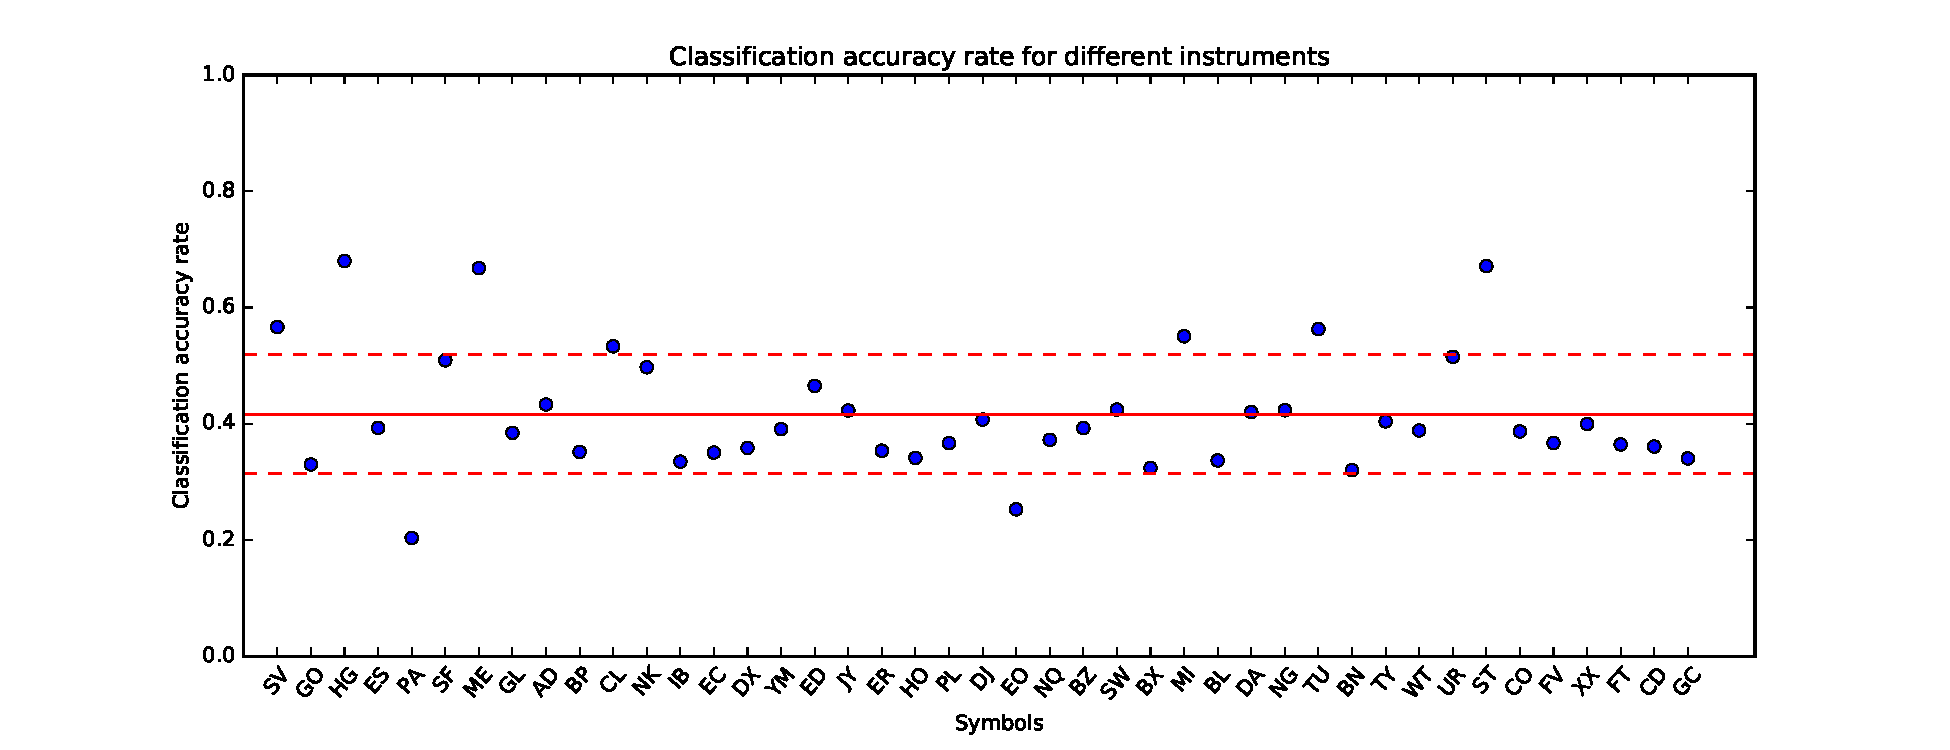
\includegraphics[width=1.3\textwidth]{figures/classification_accuracy.pdf}}
	\caption{This figure shows the classification accuracy of the DNN applied to 45 CME Commodity and FX futures. The mean and the standard deviation envelope are also shown.}
	\label{fig:classification}
\end{figure}


Figure \ref{fig:classification_accu} below shows the distribution of the average classification accuracy over 10 samples of the DNN across the 45 CME Commodity and FX futures. There's a heavier density around an accuracy of 0.35 which is slightly better than a random selection.

\begin{figure}[H]
  \makebox[\textwidth][c]{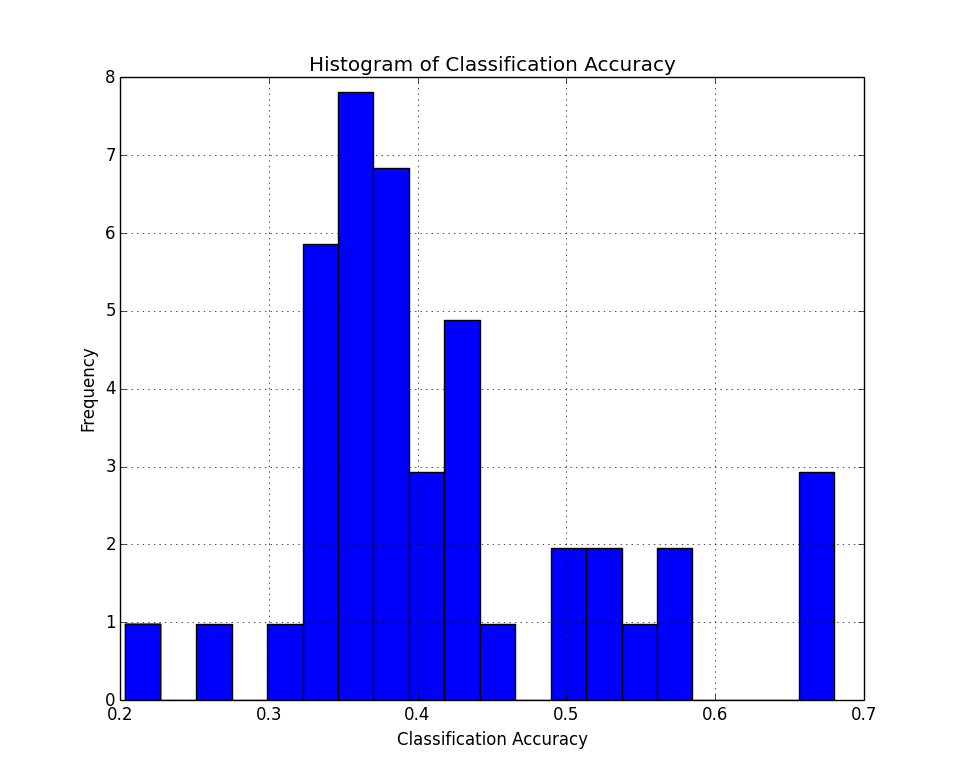
\includegraphics[width=\textwidth]{figures/hist_Classification_Accuracy.png}}
	\caption{This figure shows the distribution of average classification accuracy of the DNN applied to 45 CME Commodity and FX futures.}
	\label{fig:classification_accu}
\end{figure}


\vspace{10pt}
Table \ref{fig:top-five} shows the top five instruments for which the sample mean of the classification rate was highest on average over the ten walk forward experiments. Also shown are the F1-scores ('harmonic means') which are considered to be a more robust measure of performance due to less sensitivity to class imbalance than classification accuracies. The mean and standard deviation of the sample averaged classification accuracies and F1-scores over the 45 futures are also provided.


\vspace{10pt}
\begin{table}[h]
\centerline{
\resizebox{1.08\textwidth}{!}{
\begin{tabular}{|c|c|c|c|}
\hline
Symbol & Futures & Classification Accuracy & F1-score\\
\hline 
HG & Copper & 0.68 & 0.59\\
ST &  Transco Zone 6 Natural Gas (Platts Gas Daily) Swing& 0.67 & 0.54 \\
ME &  Gulf Coast Jet (Platts) Up-Down & 0.67 &  0.54\\
TU & Gasoil 0.1 Cargoes CIF NWE (Platts) vs. Low Sulphur Gasoil & 0.56 &  0.52\\
MI & Michigan Hub 5 MW Off-Peak Calendar-Month Day-Ahead Swap & 0.55 & 0.5 \\
\hline
mean & - & 0.42 & 0.37\\
std & -& 0.11& 0.1 \\
\hline
\end{tabular}
}}
\caption{This table shows the top five instruments for which the sample mean of the classification rate was highest over the ten walk forward experiments. F1-scores are also provided. The mean and standard deviation of the sample mean classification accuracies and F1-scores over the 45 futures are also provided.}
\label{fig:top-five}
\end{table}

\vspace{10pt}
Note that the worst five performing instruments performed no better or even worse than white noise on average over the ten experiments.






\section{Strategy Backtesting} \label{sect:backtesting}

The paper has thus far considered the predictive properties of the deep neural
network. Using commodity futures historical data at 5 minute intervals over the
period from March 31st 1991 to September 30th, 2014, this section describes the
application of a walk forward optimization approach for backtesting a simple
trading strategy.


Following the walk forward optimization approach described in \cite{Tomasini2011}, an initial optimization window of 25,000 5-minute observation periods or approximately 260 days (slightly more than a year) is chosen for training the model using all the symbol data and their engineered time series. The learning rate range is swept to find the model which gives the best out-of-sample
prediction rate - the highest classification rate on the out-of-sample ('hold-out') set consisting of 12,500 consecutive and more recent observations.

Using the optimized model, the expected P\&L of the trading strategy is then
evaluated over the out-of-sample period consisting of 12,500 consecutive 5-minute observation periods or approximately 130 days. Even though all symbols
are trained together using one DNN model, the cumulative P\&L is calculated independently for each
symbol.  As illustrated
in Figure \ref{fig:back_testing}, this step is repeated by sliding the training window forward by 1000 observation periods and repeating the out-of-sample error analysis and strategy performance measurement for ten windows.

\vspace{20pt}
\begin{figure}[h]
\centering
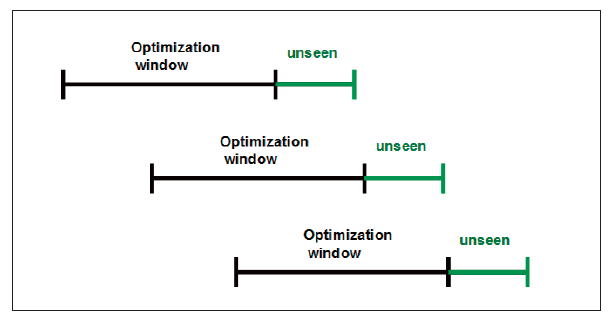
\includegraphics[scale=0.5]{figures/back_testing.png}
\caption{An illustration of the walk forward optimization method used for
backtesting the strategy}.
\label{fig:back_testing}
\end{figure}
\vspace{6pt}
\paragraph{Example trading strategy} In order to demonstrate the approach to algorithmic trading, a simple buy-hold-sell intraday test trading strategy is chosen contingent on whether the instrument price is likely to increase, be neutral, or decrease over the next
time interval respectively. For simplicity, the strategy only takes single contract positions. The strategy closes out a short position and takes a long position if the label is 1, hold the position if the label is zero and closes out the long position and takes a short position if the label is -1. In calculating the cumulative P\&L, the following assumptions are made:

\begin{itemize}
\item the account is opened with \$100k of USD;
\item there is sufficient surplus cash available in order to always maintain the brokerage account margin;
\item there are no limits on the minimum or maximum holding period and positions can be held overnight;
\item the margin account is assumed to accrue zero interest.
\item transaction costs are ignored; and
\item the market is always sufficiently liquid that a limit order gets filled at the mid-price listed at 5 minute intervals, i.e. there are no slippage effects and the bid-ask spread can be considered negligible at one lot positions.
\end{itemize}

Returns are calculated by first calculating daily returns and then annualizing them. No benchmark is used in the calculation of the Sharpe ratio.  The Capability ratio is calculated under the assumption of normality or returns. See Kumiega, Neururer and Van Vliet \cite{Vliet2014} for further details of the Capability ratio.  

Figure \ref{fig:pnl} illustrates the cumulate P\&L of the strategy for the case when perfect forecasting information is available ('test') and using the DNN prediction ('predict').  The graph is shown for one 130 day time horizon trading in PL futures. Note that the y-axis is a base 10 log scale to facilitate comparison of the 'test' and 'predict' graphs.

\begin{figure}[H]
	\makebox[\textwidth][c]{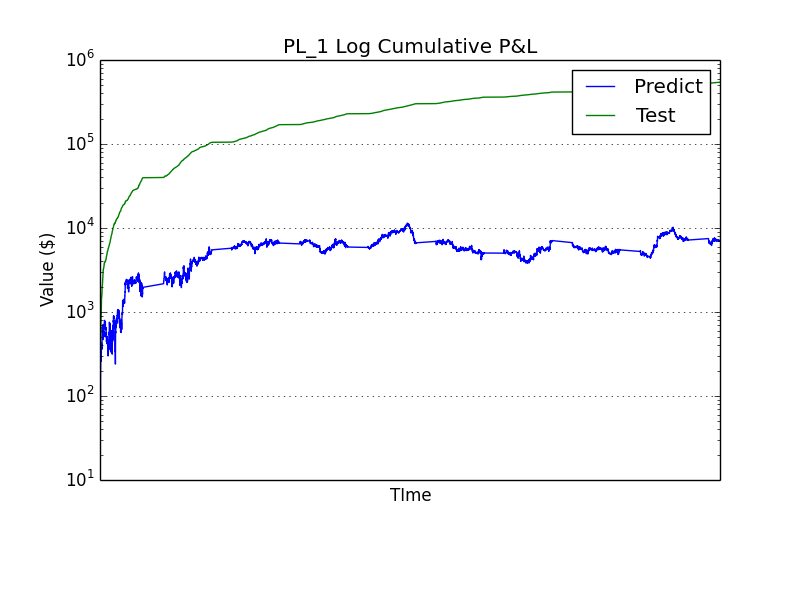
\includegraphics[width=1.2\textwidth]{figures/Log_Cum_P&L_PL_1.png}}
	\vspace{-60pt}
	\caption{This figure shows the cumulate P\&L of the strategy for the case when perfect forecasting information is available ('test') and using the DNN prediction ('predict').  The graph is shown for one 130 day time horizon trading in PL futures. Note that the y-axis is in base 10 to facilitate comparison of the 'test' and 'predict' graphs. Key: PL: Platinum, NQ: E-mini NASDAQ 100 Futures Quotes, AD: Australian Dollar, BP: British Pound, ES: E-mini S\&P 500 Futures Quotes}.
	\label{fig:pnl}
\end{figure}

Figure \ref{fig:sharpe} shows the range of annualized Sharpe ratios measured over each sliding period of 12,500 observation points for the top five performing futures contracts. This information is also supplemented in Table \ref{tab:top-five} which shows the top five instruments for which the mean annualized Shape Ratio was highest on average over the ten walk forward experiments. The values in parenthesis denote the standard deviation over the ten experiments. Also shown, are the sample mean Capability Ratios (where $n=130$) under the assumption of normality of returns and their standard deviations. 



\begin{figure}[H]
	\makebox[\textwidth][c]{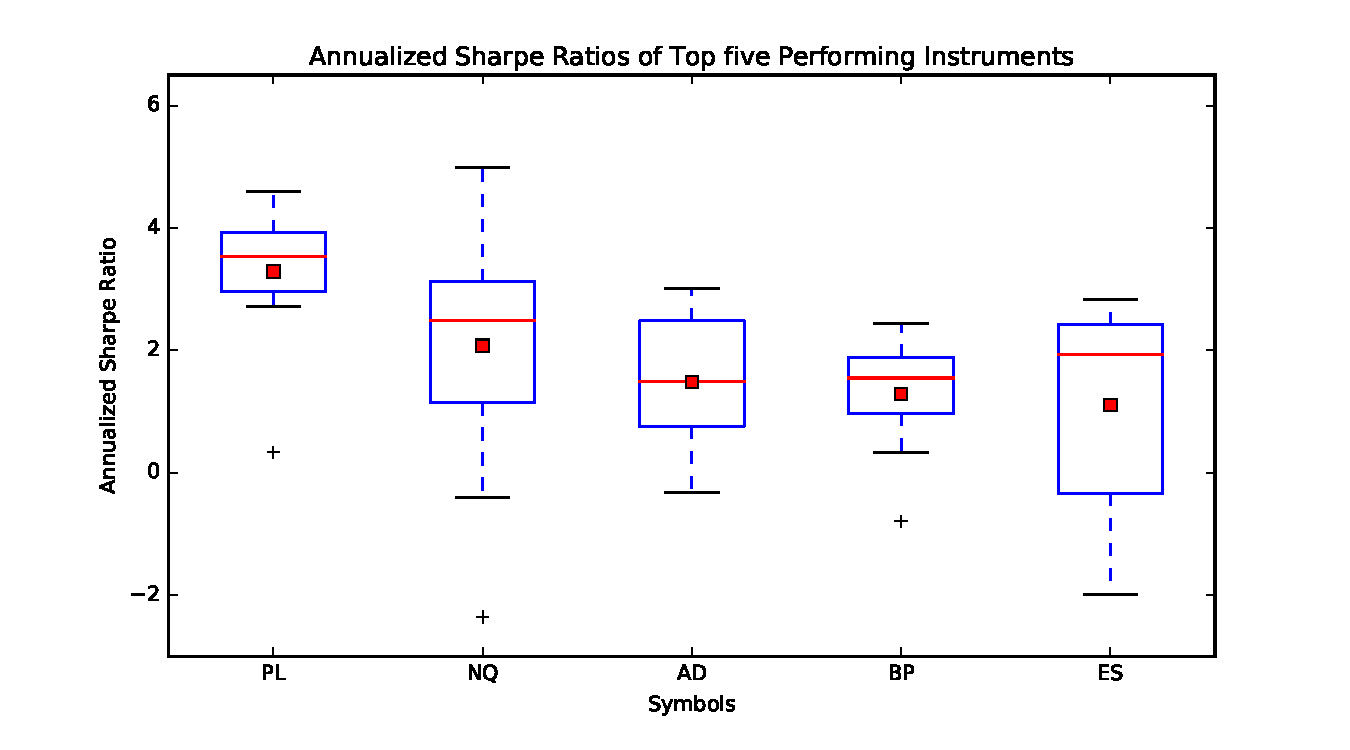
\includegraphics[width=1.2\textwidth]{figures/sharpe.pdf}}
	\caption{This figure shows the range of annualized Sharpe ratios measured over each sliding period of 12,500 observation points for the top five performing futures contracts. The simple trading strategy is described above. Key: PL: Platinum, NQ: E-mini NASDAQ 100 Futures Quotes, AD: Australian Dollar, BP: British Pound, ES: E-mini S\&P 500 Futures Quotes.}
	\label{fig:sharpe}
\end{figure}

\vspace{40pt}

\begin{table}[h]
\centerline{
\resizebox{1.05\textwidth}{!}{
\begin{tabular}{|c|c|c|c|}
\hline
Symbol & Futures & Annualized Sharpe Ratio & Capability Ratio\\
\hline 
PL & Platinum & 3.29 (1.12 ) & 12.51 (4.27) \\
NQ & E-mini NASDAQ 100 Futures Quotes& 2.07 (2.11) & 7.89 (8.03) \\
AD & Australian Dollar & 1.48 (1.09)  & 5.63 (4.13) \\
BP & British Pound & 1.29 (0.90)  &  4.90 (3.44)\\
ES & E-mini S\&P 500 Futures Quotes & 1.11 (1.69 )  & 4.22 (6.42) \\
\hline
\end{tabular}
}}
\caption{This table shows the top five instruments for which the mean annualized Shape ratio was highest on average over the ten walk forward optimizations. The values in parentheses denote the standard deviation over the ten experiments. Also shown, are the mean Capability ratios under the assumption of normality of returns and their standard deviations.}
\label{tab:top-five}
\end{table}

\vspace{30pt}

Table \ref{tab:margin} lists the initial margin, maintenance margin and contract size specified by the CME used to calculate the cumulative P\&L and strategy performance for the top five performing futures .


\begin{table}[H]
\begin{center}
\begin{tabular}{|c|c|c|c|}
\hline
Symbol &	initial margin &	maint. margin & contract size\\
\hline
PL	& 2090	&1900	&50\\
NQ	 & 5280	& 4800	& 50\\
AD	& 1980 &	1800	&100000\\
BP&	2035	 & 1850 &	62500\\
ES&	5225	& 4750&	50\\
\hline
\end{tabular}
\end{center}
\caption{This table lists the initial margin, maintenance margin and contract size specified by the CME  used to calculate the cumulative P\&L and strategy performance for the top five performing futures.}
\label{tab:margin}
\end{table}



%\clearpage
\section{Conclusion}
Deep neural networks (DNNs) are a powerful type of artificial neural network (ANN) that use several hidden layers. In this paper we describe the implementation and training of DNNs. We observe, for a historical dataset of 5 minute
mid-prices of multiple CME listed futures prices and other lags and filters that DNNs have substantial predictive capabilities as classifiers if trained concurrently across several markets on labelled data.  We further demonstrate the application of DNNs to backtesting a simple trading strategy and demonstrate the prediction accuracy and its relation to the strategy profitability. All results in this paper are generated using a C++ implementation on the Intel Xeon Phi co-processor that is 10x faster than the serial version and a python strategy backtesting environment both of which are available as open source code written by the authors.

\section{Acknowledgements} The authors gratefully acknowledge the support of Intel
Corporation in funding this research.

\clearpage
\bibliographystyle{abbrv}
\bibliography{AlgoFinance_DixonKlabjanBang} 

\end{document}
\appendix

We can obtain a sequential learning algorithm by applying the technique of
stochastic gradient descent, also known as sequential gradient descent, as follows. If
the error function comprises a sum over data points $E = \sum_{i=1}^n E_i(\mathbf{w})$,

\subsection{Recurrence}
The above formulation assumes the network topology is feed-forward where
\be
s_j^{l} = \sum_j^{d^{l-1}} w_{ij}^{l}x_i^{l-1}
\ee

We now modify the topology to include horizontal arches so that

\be \label{eq:horiz}
s_j^{l} = \sum_j^{d^{l}} w_{ij}^{l}x_i^{l-1} + s_{j-1}^{l}, ~ \forall j>1
\ee
\paragraph{Question} Equation \ref{eq:horiz} doesn't seem correct. Are there separate weights for the horizontal arches?

Additionally, we directly connect all perceptrons not connected the output layer with an additional arch so that the back-propagation formula for all layers not directly connected to the output layer becomes

\be \label{eq:bp_w_recurrence}
\delta_i^{l-1}= \sum_{j=1}^{d^{l}}\delta_j^{l} \cdot w_{ij}^{l} \cdot \sigma(s_i^{l-1})(1- \sigma(s_i^{l-1})) + \underbrace{\sum_{j=1}^{d^L}\delta_j^{L}\cdot\hat{w}_{ij}^{l}\cdot\sigma'(s_i^{l-1})}_{\text{recurrence term}}
\ee

\paragraph{Question} Is equation \ref{eq:bp_w_recurrence} the correct way to handle the extra arches between perceptrons  in layers not directly connected with outputs? Is is correct that the feed-forward step is not modified?



Evgeny Fiksman, Sania Salahuddin, "STAC-A2 on Intel Architecture: From Scalar Code to Heterogeneous Application", WHPCF, 2014, 2014 Seventh Workshop on High Performance Computational Finance (WHPCF), 2014 Seventh Workshop on High Performance Computational Finance (WHPCF) 2014, pp. 53-60



